\documentclass{article}
\usepackage[utf8]{inputenc} %кодировка
\usepackage[T2A]{fontenc}
\usepackage[english,russian]{babel} %русификатор 
\usepackage{mathtools} %библиотека матеши
\usepackage[left=1cm,right=1cm,top=2cm,bottom=2cm,bindingoffset=0cm]{geometry} %изменение отступов на листе
\usepackage{amsmath}
\usepackage{graphicx} %библиотека для графики и картинок
\graphicspath{}
\DeclareGraphicsExtensions{.pdf,.png,.jpg}
\usepackage{subcaption}
\usepackage{pgfplots}

\begin{document}
% НАЧАЛО ТИТУЛЬНОГО ЛИСТА
\begin{center}
    \Large
    Федеральное государственное автономное \\
    образовательное учреждение высшего образования \\ 
    «Научно-образовательная корпорация ИТМО»\\
    \vspace{0.5cm}
    \large
    Факультет программной инженерии и компьютерной техники \\
    Направление подготовки 09.03.04 Программная инженерия \\
    \vspace{1cm}
    \Large
    \textbf{Отчёт по лабораторной работе №4} \\
    По дисциплине «Базы данных» (второй семестр)\\
    \large
    \vspace{8cm}

    \begin{minipage}{.33\textwidth}
    \end{minipage}
    \hfill
    \begin{minipage}{.4\textwidth}
    
        \textbf{Студент}: \vspace{.1cm} \\
        \ Дениченко Александр P3112\\
        \textbf{Практик}:  \\
        \ Лисицина В.В
    \end{minipage}
    \vfill
Санкт-Петербург\\ 2023 г.
\end{center}

% КОНЕЦ ТИТУЛЬНОГО ЛИСТА 
\newpage

\section{Задание}
% 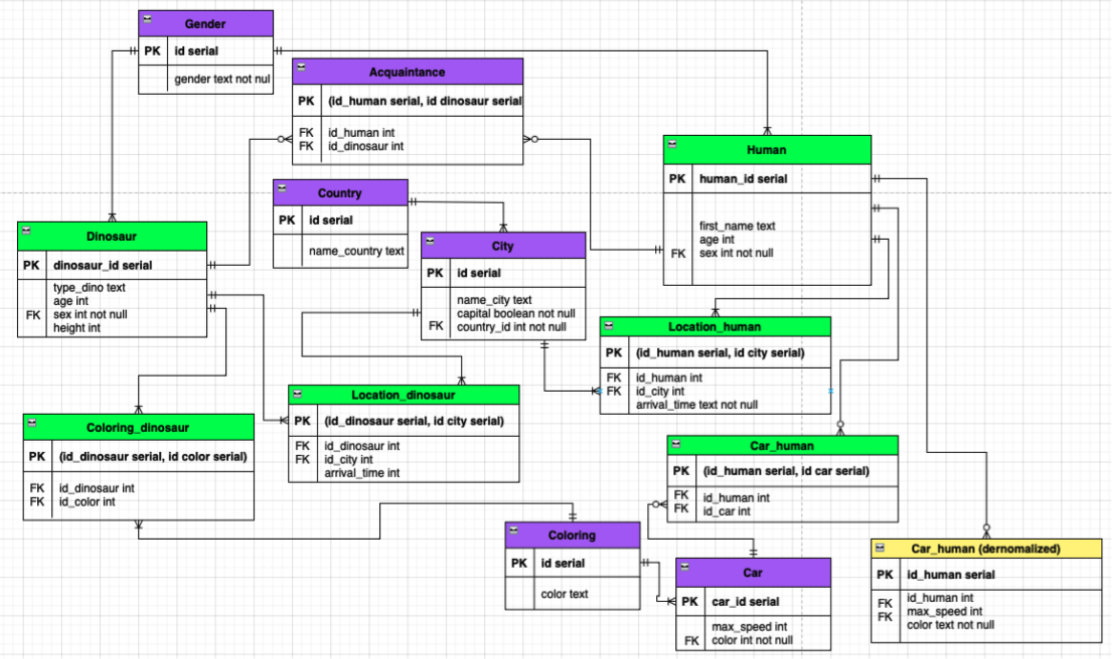
\includegraphics[width=.9\textwidth]{123}
Составить запросы на языке SQL (пункты 1-2).
\\


Для каждого запроса предложить индексы, добавление которых уменьшит время выполнения запроса (указать таблицы/атрибуты, для которых нужно добавить индексы, написать тип индекса; объяснить, почему добавление индекса будет полезным для данного запроса).
\\


Для запросов 1-2 необходимо составить возможные планы выполнения запросов. Планы составляются на основании предположения, что в таблицах отсутствуют индексы. Из составленных планов необходимо выбрать оптимальный и объяснить свой выбор.
Изменятся ли планы при добавлении индекса и как?
\\


Для запросов 1-2 необходимо добавить в отчет вывод команды EXPLAIN ANALYZE [запрос]
\\


Подробные ответы на все вышеперечисленные вопросы должны присутствовать в отчете (планы выполнения запросов должны быть нарисованы, ответы на вопросы - представлены в текстовом виде).
\\


1. Сделать запрос для получения атрибутов из указанных таблиц, применив фильтры по указанным условиям:\\
Таблицы: Н\_ЛЮДИ, Н\_СЕССИЯ.\\
Вывести атрибуты: Н\_ЛЮДИ.ФАМИЛИЯ, Н\_СЕССИЯ.ДАТА.\\
Фильтры (AND):\\
a) Н\_ЛЮДИ.ФАМИЛИЯ < Ёлкин.\\
b) Н\_СЕССИЯ.УЧГОД > 2001/2002.\\
Вид соединения: LEFT JOIN.\\


2. Сделать запрос для получения атрибутов из указанных таблиц, применив фильтры по указанным условиям:\\
Таблицы: Н\_ЛЮДИ, Н\_ОБУЧЕНИЯ, Н\_УЧЕНИКИ.\\
Вывести атрибуты: Н\_ЛЮДИ.ФАМИЛИЯ, Н\_ОБУЧЕНИЯ.НЗК, Н\_УЧЕНИКИ.ИД.\\
Фильтры: (AND)\\
a) Н\_ЛЮДИ.ОТЧЕСТВО = Сергеевич.\\
b) Н\_ОБУЧЕНИЯ.ЧЛВК\_ИД < 105590.\\
c) Н\_УЧЕНИКИ.НАЧАЛО > 2008-09-01.\\
Вид соединения: LEFT JOIN.
\section{Запросы и индексы}
1)Первый запрос:\\
\\
\begin{center}
    select Н\_ЛЮДИ.ФАМИЛИЯ, Н\_СЕССИЯ.ДАТА from Н\_ЛЮДИ\\
left outer join Н\_СЕССИЯ on Н\_ЛЮДИ.ИД = Н\_СЕССИЯ.ЧЛВК\_ИД\\
where (Н\_ЛЮДИ.ФАМИЛИЯ < 'Ёлкин' and Н\_СЕССИЯ.УЧГОД > '2001/2002');
\end{center}
Planning Time: 0.461 ms\\
Execution Time: 3.804 ms\\
\\
Для ускорения запроса можно предложить следующий вариант:\\


1.1	Для таблицы Н\_ЛЮДИ создать индекс, индексирующий столбец ФАМИЛИЯ, так как в этом отношении ФАМИЛИЯ не отсортирована, а также будем использовать кластеризованную индексацию, так как нам нужно, чтобы индекс хранил в листьях строки данных:

\begin{center}
    CREATE CLUSTERED INDEX idx\_фамилия ON Н\_ЛЮДИ USING btree(ФАМИЛИЯ);
\end{center}


1.2 Так как кластеризованной индексации нет в найшей базе данных, будем использовать только в-дерево:

\begin{center}
    CREATE INDEX idx\_фамилия ON Н\_ЛЮДИ USING btree(ФАМИЛИЯ);
\end{center}


1.3 Для таблицы Н\_СЕССИЯ никаких индексов создавать не нужно, так как количество объектов в этом отношении не слишком большое – индекс лишь замедлит процесс выборки.
\\ \\
2)Второй запрос:\\
\\
% select Н_ЛЮДИ.ФАМИЛИЯ, Н_ОБУЧЕНИЯ.НЗК, Н_УЧЕНИКИ.ИД from Н_ЛЮДИ
% left outer join Н_ОБУЧЕНИЯ on Н_ЛЮДИ.ИД = Н_ОБУЧЕНИЯ.ЧЛВК_ИД
% left outer join Н_УЧЕНИКИ on Н_ЛЮДИ.ИД = Н_УЧЕНИКИ.ЧЛВК_ИД
% where (Н_ЛЮДИ.ОТЧЕСТВО like 'Сергеевич' and Н_ОБУЧЕНИЯ.ЧЛВК_ИД < 105590 and Н_УЧЕНИКИ.НАЧАЛО
% >'2008-09-01');
\begin{center}
    select Н\_ЛЮДИ.ФАМИЛИЯ, Н\_ОБУЧЕНИЯ.НЗК, Н\_УЧЕНИКИ.ИД from Н\_ЛЮДИ\\
    left outer join Н\_ОБУЧЕНИЯ on Н\_ЛЮДИ.ИД = Н\_ОБУЧЕНИЯ.ЧЛВК\_ИД\\
    left outer join Н\_УЧЕНИКИ on Н\_ЛЮДИ.ИД = Н\_УЧЕНИКИ.ЧЛВК\_ИД\\
    where (Н\_ЛЮДИ.ОТЧЕСТВО like 'Сергеевич' and Н\_ОБУЧЕНИЯ.ЧЛВК\_ИД < 105590 and Н\_УЧЕНИКИ.НАЧАЛО >'2008-09-01');
\end{center}
Planning Time: 0.766 ms\\
Execution Time: 0.054 ms\\
\\
Для ускорения запроса можно предложить следующий вариант:\\


2.1 Для таблицы Н\_ЛЮДИ можно проиндексировать атрибут ОТЧЕСТВО:
\begin{center}
    CREATE INDEX idx\_отчество ON Н\_ЛЮДИ USING btree(ОТЧЕСТВО);
\end{center}


2.2 Для таблицы Н\_ОБУЧЕНИЯ можно проиндексировать атрибут ЧЛВК\_ИД, так как в условии WHERE используется неравенство, то выборку мы можем ускорить при помощи B-дерева:
\begin{center}
    CREATE INDEX idx\_ид\_обуч ON Н\_ОБУЧЕНИЯ USING btree(ЧЛВК\_ИД);
\end{center}


2.3 Для таблицы Н\_УЧЕНИКИ можно проиндексировать атрибут НАЧАЛО, так как в условии WHERE используется неравенство, то выборку мы можем ускорить при помощи B-дерева:
\begin{center}
    CREATE INDEX idx\_начало ON Н\_УЧЕНИКИ USING btree(НАЧАЛО);
\end{center}

\section{Планы выполнения}
1)Первый запрос:\\



    3.1 Неоптимальный план выполнения:\\
    \begin{center}
        \begin{tikzpicture}[level distance=1.2cm,
            level 1/.style={sibling distance=2cm},
            level 2/.style={sibling distance=5cm}]
              \node {result}
              child {node {$\pi$ Н\_ЛЮДИ.ФАМИЛИЯ Н\_СЕССИЯ.ДАТА}
                child {node {$\sigma $ Н\_ЛЮДИ.ФАМИЛИЯ < Ёлкин}
                child {node {$\sigma $ Н\_СЕССИЯ.УЧГОД > 2001/2002}
                child {node {$\bowtie$ Н\_ЛЮДИ.ИД = Н\_СЕССИЯ.ЧЛВК\_ИД}
                child {node {Н\_ЛЮДИ }}
                child {node {Н\_СЕССИЯ}}
              }}}};
        \end{tikzpicture}
    \end{center}
3.2 Оптимальный план выполнения: 
\\Целью оптимизации является уменьшение размеров промежуточных данных -> уменьшение числа операций чтения записи во внешнюю память
\begin{center}
    \begin{tikzpicture}[level distance=1.2cm,
        level 1/.style={sibling distance=2cm},
        level 2/.style={sibling distance=8cm}]
          \node {result}
          child {node {$\pi$ Н\_ЛЮДИ.ФАМИЛИЯ Н\_СЕССИЯ.ДАТА}
            child {node {$\bowtie$ Н\_ЛЮДИ.ИД = Н\_СЕССИЯ.ЧЛВК\_ИД}
            child {node {$\sigma $ Н\_ЛЮДИ.ФАМИЛИЯ < Ёлкин} child {node {Н\_ЛЮДИ }}}
            child {node {$\sigma $ Н\_СЕССИЯ.УЧГОД > 2001/2002} child {node {Н\_СЕССИЯ}}}
            }};
    \end{tikzpicture}
\end{center}
Этот план выполнения оптимален так как мы достигли цели. На момент соединения строк перебор будет минимальным за счёт отдельных процессов выборки, получилось разделение процессов.
\\ \\
2)Второй запрос:\\


    4.1 Неоптимальный план выполнения:\\
    \begin{center}
        \begin{tikzpicture}[level distance=1.2cm,
            level 1/.style={sibling distance=2cm},
            level 2/.style={sibling distance=5cm}]
              \node {result}
              child {node {$\pi$  Н\_ЛЮДИ, Н\_ОБУЧЕНИЯ, Н\_УЧЕНИКИ}
                child {node {$\sigma $ Н\_УЧЕНИКИ.НАЧАЛО > 2008-09-01}
                child {node {$\sigma $ Н\_ОБУЧЕНИЯ.ЧЛВК\_ИД < 105590}
                child {node {$\sigma$ Н\_ЛЮДИ.ОТЧЕСТВО = Сергеевич}
                child {node {$\bowtie$ Н\_ЛЮДИ.ИД = Н\_ОБУЧЕНИЯ.ЧЛВК\_ИД $\wedge$ Н\_ЛЮДИ.ИД = Н\_УЧЕНИКИ.ЧЛВК\_ИД}
                child {node {Н\_ЛЮДИ }}
                child {node {Н\_ОБУЧЕНИ}}
                child {node {Н\_УЧЕНИКИ}}
              }}}}};
        \end{tikzpicture}
    \end{center}
4.2 Средне - оптимальный план выполнения: 
\\Целью оптимизации является уменьшение размеров промежуточных данных -> уменьшение числа операций чтения записи во внешнюю память
\begin{center}
    \begin{tikzpicture}[level distance=1.2cm,
        level 1/.style={sibling distance=2cm},
        level 2/.style={sibling distance=6.8cm}]
          \node {result}
          child {node {$\pi$  Н\_ЛЮДИ, Н\_ОБУЧЕНИЯ, Н\_УЧЕНИКИ}
          child {node {$\bowtie$ Н\_ЛЮДИ.ИД = Н\_ОБУЧЕНИЯ.ЧЛВК\_ИД $\wedge$ Н\_ЛЮДИ.ИД = Н\_УЧЕНИКИ.ЧЛВК\_ИД}
            child {node {$\sigma $ Н\_УЧЕНИКИ.НАЧАЛО > 2008-09-01}child {node {Н\_УЧЕНИКИ}}}
            child {node {$\sigma $ Н\_ОБУЧЕНИЯ.ЧЛВК\_ИД < 105590}
            child {node {Н\_ОБУЧЕНИ}}}
            child {node {$\sigma$ Н\_ЛЮДИ.ОТЧЕСТВО = Сергеевич}
            child {node {Н\_ЛЮДИ }}
          }}};
    \end{tikzpicture}
\end{center}
Этот план выполнения средне - оптимальный так как мы достигли цели, но для подобных планов лучше использовать левостороннее дерево, где выборка будет происходить перед каждым соединением, что упростит поиск подходящих объектов.
\\ \\

4.2 Оптимальный план выполнения: 
\begin{center}
    \begin{tikzpicture}[level distance=1.2cm,
        level 1/.style={sibling distance=2cm},
        level 2/.style={sibling distance=10cm},
        level 3/.style={sibling distance=10cm},
        level 4/.style={sibling distance=7cm}]
          \node {result}
          child {node {$\pi$  Н\_ЛЮДИ, Н\_ОБУЧЕНИЯ, Н\_УЧЕНИКИ}
          child {node {$\bowtie$ Н\_ЛЮДИ.ИД = Н\_УЧЕНИКИ.ЧЛВК\_ИД }
          child {node {$\bowtie$ Н\_ЛЮДИ.ИД = Н\_ОБУЧЕНИЯ.ЧЛВК\_ИД }
            child {node {$\sigma$ Н\_ЛЮДИ.ОТЧЕСТВО = Сергеевич}
            child {node {Н\_ЛЮДИ }}}
            child {node {$\sigma $ Н\_ОБУЧЕНИЯ.ЧЛВК\_ИД < 105590}
            child {node {Н\_ОБУЧЕНИ}}}
            }
            child {node {$\sigma $ Н\_УЧЕНИКИ.НАЧАЛО > 2008-09-01}child {node {Н\_УЧЕНИКИ}}}
            }};
    \end{tikzpicture}
\end{center}
5.1 Влияние на план выборки индексами:
\\ \\ 5.2 Если запрос содержит условие, которое может быть поддержано созданным индексом, это может привести к более быстрому выполнению операции поиска. База данных может использовать индекс для быстрого нахождения соответствующих строк, что улучшит производительность запроса.
\\ \\ 5.3 Вместо сортировки всей таблицы, база данных может использовать индекс для получения данных уже отсортированными, что может значительно ускорить выполнение запроса.
\\ \\ 5.4 При выполнении операции объединения таблиц, наличие соответствующих индексов может улучшить производительность. База данных может использовать индексы для быстрого нахождения соответствующих строк и выполнения объединения.
\\ \\ 5.5 Добавление индекса может изменить стоимость выполнения различных операций в базе данных. Планировщик запросов может выбрать новый план выполнения, учитывая наличие индексов и их стоимость. В некоторых случаях это может привести к изменению порядка выполнения операций или выбору других типов доступа к данным.
\section{EXPLAIN ANALYZE}
Запрос первый:
\begin{center}
    EXPLAIN ANALYZE select Н\_ЛЮДИ.ФАМИЛИЯ, Н\_СЕССИЯ.ДАТА from Н\_ЛЮДИ\\
left outer join Н\_СЕССИЯ on Н\_ЛЮДИ.ИД = Н\_СЕССИЯ.ЧЛВК\_ИД\\
where (Н\_ЛЮДИ.ФАМИЛИЯ < 'Ёлкин' and Н\_СЕССИЯ.УЧГОД > '2001/2002');
\end{center}
Answer:\\
\\
    Nested Loop  (cost=0.29..286.49 rows=826 width=24) (actual time=0.067..3.782 rows=937 loops=1)
    \\->  Seq Scan on "Н\_СЕССИЯ"  (cost=0.00..117.90 rows=3630 width=12) (actual time=0.014..1.887 rows=3630 loops=1)
         \\ Filter: (("УЧГОД")::text > '2001/2002'::text)
          \\Rows Removed by Filter: 122
    \\->  Memoize  (cost=0.29..0.44 rows=1 width=20) (actual time=0.000..0.000 rows=0 loops=3630)
         \\ Cache Key: "Н\_СЕССИЯ"."ЧЛВК\_ИД"
        \\  Cache Mode: logical
        \\  Hits: 3452  Misses: 178  Evictions: 0  Overflows: 0  Memory Usage: 15kB
        \\  ->  Index Scan using "ЧЛВК\_PK" on "Н\_ЛЮДИ"  (cost=0.28..0.43 rows=1 width=20) (actual time=0.003..0.003 rows=0 loops=178)
         \\       Index Cond: ("ИД" = "Н\_СЕССИЯ"."ЧЛВК\_ИД")
          \\      Filter: (("ФАМИЛИЯ")::text < 'Ёлкин'::text)
           \\     Rows Removed by Filter: 1
  \\Planning Time: 0.398 ms
  \\Execution Time: 3.870 ms
 (14 строк)\\
 \\ \\
 Запрос второй:
 \begin{center}
    explain analyze select Н\_ЛЮДИ.ФАМИЛИЯ, Н\_ОБУЧЕНИЯ.НЗК, Н\_УЧЕНИКИ.ИД from Н\_ЛЮДИ
    \\left outer join Н\_ОБУЧЕНИЯ on Н\_ЛЮДИ.ИД = Н\_ОБУЧЕНИЯ.ЧЛВК\_ИД
    \\left outer join Н\_УЧЕНИКИ on Н\_ЛЮДИ.ИД = Н\_УЧЕНИКИ.ЧЛВК\_ИД
    \\where (Н\_ЛЮДИ.ОТЧЕСТВО like 'Сергеевич' and Н\_ОБУЧЕНИЯ.ЧЛВК\_ИД < 105590 and Н\_УЧЕНИКИ.НАЧАЛО
    \\>'2008-09-01');
 \end{center}
 Answer:\\
 \\Nested Loop  (cost=0.85..21.42 rows=1 width=26) (actual time=0.006..0.006 rows=0 loops=1)
 \\->  Nested Loop  (cost=0.56..15.22 rows=1 width=30) (actual time=0.005..0.006 rows=0 loops=1)
       \\->  Index Scan using "ОБУЧ\_ЧЛВК\_FK\_I" on "Н\_ОБУЧЕНИЯ"  (cost=0.28..6.87 rows=1 width=10) (actual time=0.005..0.005 rows=0 loops=1)
       \\      Index Cond: ("ЧЛВК\_ИД" < 105590)
     \\  ->  Index Scan using "ЧЛВК\_PK" on "Н\_ЛЮДИ"  (cost=0.28..8.30 rows=1 width=20) (never executed)
      \\       Index Cond: ("ИД" = "Н\_ОБУЧЕНИЯ"."ЧЛВК\_ИД")
      \\       Filter: (("ОТЧЕСТВО")::text ~~ 'Сергеевич'::text)
\\ ->  Index Scan using "УЧЕН\_ОБУЧ\_FK\_I" on "Н\_УЧЕНИКИ"  (cost=0.29..6.20 rows=1 width=8) (never executed)
  \\     Index Cond: ("ЧЛВК\_ИД" = "Н\_ЛЮДИ"."ИД")
  \\     Filter: ("НАЧАЛО" > '2008-09-01 00:00:00'::timestamp without time zone)
\\Planning Time: 0.687 ms
\\Execution Time: 0.055 ms
\\(12 строк)
\section{Вывод}
1. Индексы играют важную роль в оптимизации запросов, ускоряя операции поиска, сортировки и объединения таблиц.
\\2. При добавлении индексов могут измениться планы выполнения запросов, что может улучшить производительность.
\\3. Выбор типа индекса зависит от структуры таблицы и операций над данными.
\\4. Необходимо проводить анализ производительности и тестирование изменений с индексами.
\\5. Оптимизация производительности базы данных - сложная задача, требующая учета множества факторов.


\end{document}

